\documentclass[10pt,a4paper]{amsart}
\usepackage[margin=19mm]{geometry}
\usepackage{amsmath,amssymb,mathtools}
\usepackage[scr=rsfs,cal=euler]{mathalfa}
\usepackage{xfrac}
\usepackage[unicode,hidelinks,bookmarks=false]{hyperref}
\newcommand{\ie}{i.e.\ }
\newcommand{\cf}{cf.\ }
\newcommand{\resp}{respectively\ }
\newcommand{\Subsection}{\subsection}
\providecommand{\nobreakdash}{\nobreak\hbox{-}}
\setlength{\emergencystretch}{2em}
\multlinegap0pt
\usepackage{tikz}
\usepackage{mathtools}
\usepackage{amssymb}
\newtheorem{remark}{Remark}
\newtheorem{prop}{Proposition}
\title{Frobenius--Witt cotangent complexes}
\author{Kanau Shimada}
\date{Source: arXiv:2605.14803v3 (CC BY 4.0)}
\begin{document}
\maketitle

\noindent\emph{Source and licence.} Frobenius--Witt cotangent complexes. Version arXiv:2605.14803v3 (CC BY 4.0), distributed by arXiv under the Creative Commons Attribution 4.0 International licence, http://creativecommons.org/licenses/by/4.0/, as recorded in the arXiv licence metadata for this exact version and shown on the abstract page https://arxiv.org/abs/2605.14803v3. Full licence notice: \texttt{licenses/arxiv-2605.14803-CC-BY-4.0.txt}.\par\smallskip

\noindent\textit{Editorial scope.} Counted unit: the article's prop pro4.10.1 (source0.tex lines 527--532). The article's complete original proof of it is delivered with it (source0.tex lines 533--553, one \texttt{proof} environment of 21 lines). No mathematics is written, repaired or re-derived: the statement and the proof are the article's own lines, in the article's own notation, and no retained line is substituted or re-flowed.  Retained uncounted as the source-local context the proof needs: lines 466--472; lines 511--513.  Nothing was omitted from any retained span, so the package carries no omission record.  No retained line contains a citation, so the wrapper carries no bibliography and no bibliography entry.  The retained lines contain the article's own diagram code, which the wrapper typesets with the standard tikz packages; no image file is delivered and the package declares no asset dependency.  Editorial formatting only, in addition: an AMS \texttt{amsart} preamble that restates the article's own declarations and macros used by the retained lines, namely the environments \texttt{remark}, \texttt{prop} on separate counters, together with the standard packages those lines need.  The retained environments print in this document as Remark 1, Proposition 1 in order of appearance, whereas the article prints the same items with the numbering of its own full document.  The complete native source of the article as distributed in the arXiv e-print for this exact version is bundled unchanged as \texttt{sources/200613/source0.tex}.
\begin{remark}\label{rem4.2}
    \begin{enumerate}
        \item We denote by $\mathrm{pr}_1:W^{\mathrm{an}}(A,M,m)\to R$ the natural transformation defined by the animation of the natural transformation $W(R,M,m)\to R:(a,x)\mapsto a$. Remark that this is a map of animated rings.
        \item We denote by $\mathrm{pr}_2:W^{\mathrm{an}}(A,M,m)\to M$ the natural transformation defined by the animation of the natural transformation $W(R,M,m)\to M:(a,x)\mapsto x$. Remark that this is only a map of spaces.
        \item Let $(\mathrm{pr}_1,\mathrm{pr}_2):W_2(R,M,m)\to R\times M$ be the map of spaces induced by $\mathrm{pr}_1$ and $\mathrm{pr}_2$. Since this functor preserves all sifted colimits by definition, it coincides with the animation of the functor \[\operatorname{AlgMod_*^{p-tor}}\to \operatorname{Set}:(A,M,m)\mapsto A\times M.\]  It follows from this observation and the canonical isomorphism $W_2(A,M,m)\xrightarrow[]{\cong}A\times M$ for each discrete object $(A,M,m)$ that there exists a natural equivalence \[W_2^{an}(A,M,m)\xrightarrow[]{\simeq } A\times M\] of spaces for all $(A,M,m)\in \operatorname{Ani(RingMod_*^{p-tor})}$.
    \end{enumerate}
\end{remark}

\begin{prop}\label{pro4.8.1}
    The construction $A\mapsto (A,F\mathbb L_A,\widetilde m)$ defines a functor \[\operatorname{Ani(Ring)}_{\mathbb Z_{(p)}/}\to \operatorname{Ani(AlgMod_{*}^{p-tor})}:A\mapsto (A,F\mathbb L_A,\widetilde m)\] of $\infty$-categories.
\end{prop}

\begin{prop}\label{pro4.10.1}
    The functor \[\operatorname{Ani(Ring)}_{\mathbb Z_{(p)}/}\to \operatorname{Ani(AlgMod_{*}^{p-tor})}:A\mapsto (A,F\mathbb L_A,\widetilde m)\] commutes with all sifted colimits and pushouts.

    In particular, the functor 
    \[\operatorname{Ani(Ring)}_{\mathbb Z_{(p)}/}\to \mathcal D(\mathbb F_p)\] commutes with all sifted colimits and pushouts.
\end{prop}

\begin{proof}
Let $\{A_i\}_{i\in I}$ be an arbitrary sifted or pushout diagram in $\operatorname{Ani(Ring)}_{\mathbb Z_{(p)}/}$. Denote by $A$ its colimit. By functoriality (Proposition\ref{pro4.8.1}), there exists a canonical map $\operatorname{colim}_{i\in I}(F\mathbb L_{A_i}\otimes^L_{A_i}A)\to F\mathbb L_A$. For any $(M,m)\in \mathcal D(A/^Lp)_{(A/^Lp)/}$, we have the following equivalences in $\mathcal S$:\begin{align*}
    \operatorname{Hom}_{\mathcal D(A/^Lp)_{(A/^Lp)/}}(\operatorname{colim}_{i\in I}(F\mathbb L_{A_i}\otimes^L_{A_i}A),M)&\simeq \operatorname{lim}_{i\in I}\operatorname{Hom}_{\mathcal D(A/^Lp)_{(A/^Lp)/}}(F\mathbb L_{A_i}\otimes^L_{A_i}A,M)\\
    &\simeq \operatorname{lim}_{i\in I}\operatorname{FWDer}(A_i,M)\\
    &\simeq \operatorname{lim}_{i\in I}\operatorname{Hom}_{\operatorname{Ani(Ring)}_{\mathbb Z_{(p)}//A_i}}(A_i,W_2(A_i,M))\\
    &\simeq \operatorname{lim}_{i\in I}\operatorname{Hom}_{\operatorname{Ani(Ring)}_{\mathbb Z_{(p)}//A}}(A_i,W_2(A,M))\\
    &\simeq \operatorname{Hom}_{\operatorname{Ani(Ring)}_{\mathbb Z_{(p)}//A}}(\operatorname{colim}_{i\in I} A_i,W_2(A,M))\\
    &\simeq \operatorname{FWDer}(A,M)\\
    &\simeq \operatorname{Hom}_{\mathcal D(A/^Lp)_{(A/^Lp)/}}(F\mathbb L_A,M), 
\end{align*}
where, for simplicity of notation, we write $N$ for an object $(N,n)$ of $\mathcal D(A/^Lp)_{(A/^Lp)/}$. Remark that in the 4-th equivalence in the above computation, we used the fact that the following diagram of animated rings is a pullback square:
\[ 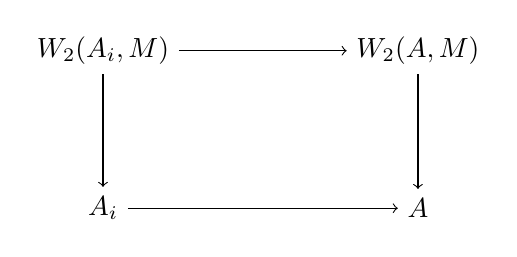
\begin{tikzpicture}[auto]
\node (a) at (0, 2) {$W_2(A_i,M)$}; \node (x) at (4, 2) {$W_2(A,M)$};
\node (b) at (0, 0) {$A_i$};   \node (y) at (4, 0) {$A$};
\draw[->] (a) to node {$\scriptstyle $} (x);
\draw[->] (x) to node {$\scriptstyle $} (y);
\draw[->] (a) to node[swap] {$\scriptstyle $} (b);
\draw[->] (b) to node[swap] {$\scriptstyle $} (y);
\end{tikzpicture},\]
which follows from (3) of Remark \ref{rem4.2}. Thus we proved the proposition.
\end{proof}

\end{document}
